\documentclass[%
% aspectratio=169
]{beamer}

\usetheme{Janelia}

\usepackage{amssymb}% http://ctan.org/pkg/amssymb

\usepackage{graphicx}

\usepackage{hyperref}
\hypersetup{colorlinks,linkcolor=,urlcolor=HHMIGreenB}

\usepackage{pygmentex}

\usepackage{tikz}
\usetikzlibrary{calc}
\usetikzlibrary{decorations}
\usetikzlibrary{decorations.pathmorphing}
\usetikzlibrary{decorations.text}
\usetikzlibrary{patterns}
\usetikzlibrary{shapes.misc}
\usepgflibrary{decorations.pathmorphing}

\usepackage{pifont}% http://ctan.org/pkg/pifont
\newcommand{\cmark}{\ding{51}}%
\newcommand{\xmark}{\ding{55}}%
\newcommand{\rxmark}{\color{red}\xmark}

\usepackage{tabulary}

% \addtobeamertemplate{footnote}{}{\vspace{2ex}}

\title[imglyb]{imglyb\\[0.3em]Bridging The Chasm Between ImageJ and NumPy}
\subtitle{imglyb}
\author{Philipp Hanslovsky}
\date{July 10, 2019}

% \setcounter{showSlideNumbers}{1}

\usepackage{sourceserifpro}
\usepackage{sourcesanspro}
\usepackage{sourcecodepro}

\usepackage{listings}
\lstset{
    basicstyle=\ttfamily\scriptsize
}

\newcommand{\urlScrSz}[1]{\scriptsize\url{#1}}

\begin{document}

% \setcounter{showProgressBar}{0}
% \setcounter{showSlideNumbers}{0}

\maketitle
% Tell story: About five 1/2 years ago I moved from Heidelberg, Germany all the way across the
% Atlantic to Ashburn, VA, just outside Washington DC. After arrival I learned that I would have a
% much bigger journey still ahead of me.

% \section{Introduction}
\begin{frame}
    \frametitle{}
    % Tell story: I first started programming seriously during my Master's
    % when I worked on cell tracking in developing embryos in the Hamprecht lab at Heidelberg
    % University. The lab was and is still creating high-performance software in C++ and with Python
    % wrappers for easy interaction. Naturally, I was exposed to C++ and Python, in particular the
    % NumPy and SciPy frameworks as depicted here as Mount SciPy. It took a lot learning and effort
    % but eventually I managed to climb Mount SciPy and was comfortable writing software in
    % the SciPy framework. The wealth of concise array arithmetic and scientific libraries help
    % developers create efficient software with a minimal number of lines of very readable code.
        \centering
    \vfill
    \begin{tikzpicture}[x=\textwidth, y=\textheight]
        \pgfmathsetseed{23654}
        \fill[brown, draw=black]
        decorate [decoration={random steps, segment length=5pt, amplitude=1.5pt}]%
        {
            (0,0) -- (0.1, 0.12) -- (0.2, 0.2)-- (0.4,0.5) -- (0.46, 0.12) -- (0.5,0.04) --
            (0.52, 0.14) -- (0.57, 0.5) -- (0.59, 0.49) -- (0.65, 0.3) -- (1,0)
        }%
        -- cycle;

        \visible<2->{
            \node[] at (.17,0.48) {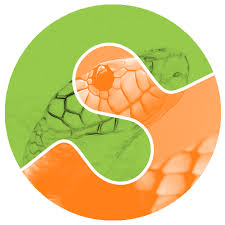
\includegraphics[height=0.075\textwidth]{fig/logos/python/scikit-image.jpeg}};
            \node[] at (.34,0.54) {
\includegraphics[height=0.075\textwidth]{fig/logos/python/scipy.png}};
            \node[] at (.2,0.565) {
\includegraphics[height=0.025\textwidth]{fig/logos/python/matplotlib.pdf}};
            \node[] at (.22,0.39) {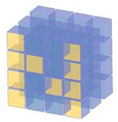
\includegraphics[height=0.075\textwidth]{fig/logos/python/numpy.png}};
        }
        \visible<2->{\node[] at (.28,0.48) {
\includegraphics[height=0.09\textwidth]{fig/logos/python/python.png}};}
        
        \visible<3->{
            \node[] at (.735,0.53) {
\includegraphics[height=0.075\textwidth]{fig/logos/imagej/trackmate.png}};
            \node[] at (.735,0.45) {
\includegraphics[height=0.075\textwidth]{fig/logos/imagej/fiji.png}};
            \node[] at (.658,0.375) {
\includegraphics[height=0.075\textwidth]{fig/logos/imagej/mammut.png}};
            \node[] at (.59,0.54) {
\includegraphics[height=0.075\textwidth]{fig/logos/imagej/imglib2.png}};
        }
        \visible<3->{\node[] at (.65,0.48) {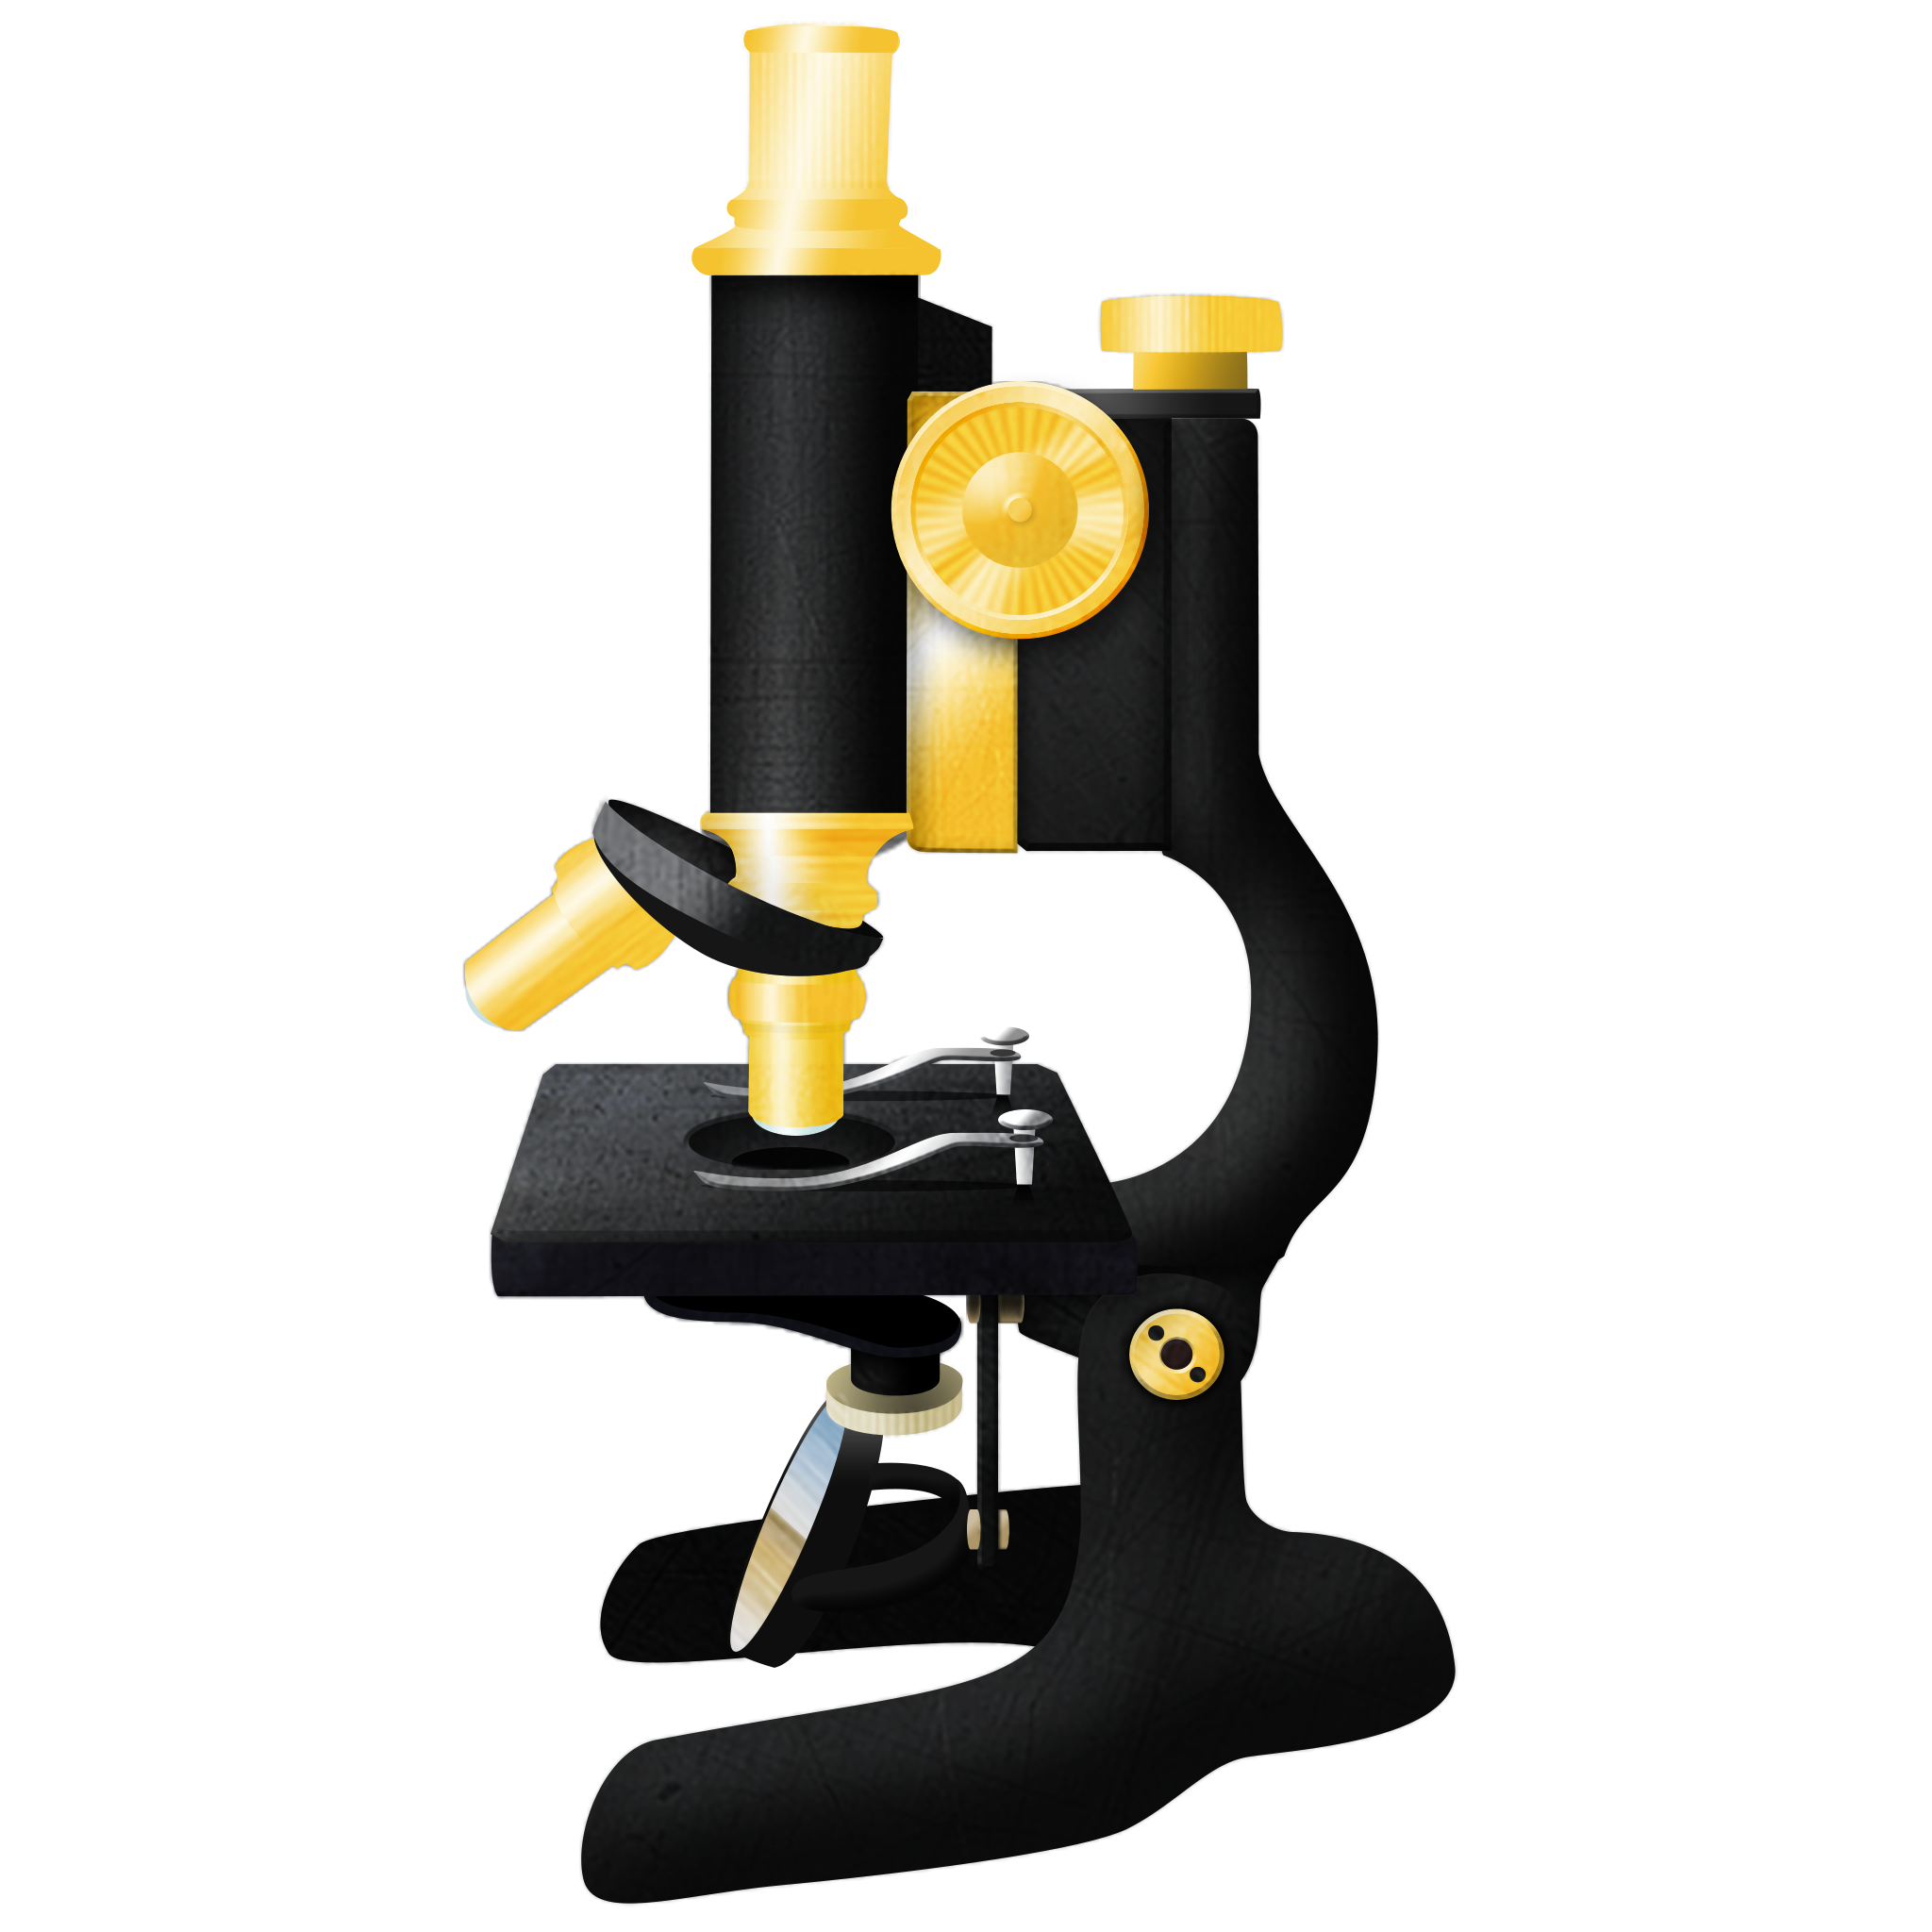
\includegraphics[height=0.13\textwidth]{fig/logos/imagej/imagej2.png}};}

        % \visible<6->{
        %     % source https://openclipart.org/detail/209218/firebog-bridge
        %     \node[anchor=south west] at (0.38, 0.41) {
\includegraphics[width=0.19\linewidth]{fig/bridge.pdf}};
        % }
        
    \end{tikzpicture}

    % After my move to the US, I realized that not everybody is doing in Image Processing in C++ or
    % Python: For the first time in my life, I had to program in the Java programming
    % language. Contrary to popular misconception, image processing can be very efficient in Java, but
    % it is very different than in Python. I had to climb another mountain, Mount ImgLib2, and many
    % times I stumbled and fell down because previously learned patterns in the SciPy environment were
    % not valid anymore. After a long but successful ascent, I finally understood and learned to
    % appreciate the design: Pixel access is virtualized and independent from how the data is
    % provided: For example, as Java arrays, chunked images, or as a function of the
    % coordinate. Sometimes I find myself on top of Mount ImgLib2 happily coding away and then I look
    % over to Mount SciPy and I can see all the neat SciPy libraries and Python features like operator
    % overloading for concise notation of array operations. Mount SciPy seems so close but there is
    % this huge chasm in between that separates those two peaks. I created imglyb to bridge this
    % chasm for shared memory access of NumPy and ImgLIb2 data structures.

\end{frame}

\begin{frame}
    \frametitle{Contents}
    \begin{enumerate}
          \item Why is shared memory hard?
          \item Solution
          \item Examples
          \item Known issues
    \end{enumerate}
\end{frame}

\begin{frame}
    \frametitle{What is Python?}
    \begin{itemize}
          \item<1-> Interpreted language with dynamic typing.
          \item<2-> Access to native memory.
          \item<3-> Efficient software through C/C++ extensions.
          \item<4-> Interactive shell and notebooks.
    \end{itemize}
\end{frame}

\begin{frame}
    \frametitle{What is Java?}
    \begin{itemize}
          \item<1-> Statically typed language that compiles into byte code.
          \item<2-> Byte code is executed within a virtual machine (JVM).
          \item<3-> No access to native memory through Java language API.
    \end{itemize}
\end{frame}

% \section{imglyb}
\begin{frame}
    \frametitle{Why are they hard to combine?}
    \begin{itemize}
          \item Native vs JVM
          \item Java Array $\neq$ C-Array
    \end{itemize}
\end{frame}

\begin{frame}
    \frametitle{Ways out of the dilemma}
    \begin{itemize}
          \item<1-> Inter-process communication:
        \begin{itemize}
              \item<2->[\cmark] Comparatively easy.
              \item<2->[\cmark] Can be extended to any language.
              \item<2->[\rxmark] No shared memory.
        \end{itemize}
        \item[]
        \item<3-> Python and JVM in the same process:
      \begin{itemize}
            \item<4->[\cmark] Shared memory possible.
            \item<4->[\cmark] Avoids unnecessary copies of data.
      \end{itemize}

      \visible<5->{
          
\begin{tikzpicture}[overlay]
              % \draw[decorate,thick] (0,0) -- (0,3) -- (3,3);
              \draw[decorate,ultra thick, green, rounded corners=0] (-0.5,0.2) rectangle (8,2);
              % \draw[decorate,ultra thick] (0,0) ellipse (3,3);
          \end{tikzpicture}
      }
        %   \item Py4j: Independent Java and Python processes communicate~--- no shared memory
        %   \item Start Python process within Java and expose Python classes through JNI: Cool but
        % cannot use Python syntax like operator overloading
        %   \item JyNI Re-implement Python in Java~(Jython) and make CPython libraries accessible through JNI:
        % Jython only 2.7
        %   \item Start a JVM in Python process through JNI and make native memory accessible in ImgLib2 
    \end{itemize}
\end{frame}

\begin{frame}
    \frametitle{Two options}
    \begin{itemize}
          \item<1-> Java implementation of Python: Jython %\footnote{\urlScrSz{https://www.jython.org/}}
        \begin{itemize}
              \item<2->[\cmark] Access native CPython extensions through Jython Native Interface
              \item<3->[\rxmark] Only Jython 2.7 is available
        \end{itemize}
          \item<4-> Start Java within a CPython process
    \end{itemize}
          \visible<4->{
          \begin{tikzpicture}[overlay]
              % \draw[decorate,thick] (0,0) -- (0,3) -- (3,3);
              \draw[decorate,ultra thick, green, rounded corners=0] (-0.5,0.4) rectangle (8,1.0);
              % \draw[decorate,ultra thick] (0,0) ellipse (3,3);
          \end{tikzpicture}
      }
\end{frame}


\begin{frame}
    \frametitle{Way out!}
    \begin{itemize}
        \setlength{\itemindent}{-0.5cm}
          \item<1->[\only<1->{\color{green}\cmark}] Start JVM from Python process.
        \begin{itemize}
        \setlength{\itemindent}{-1.0cm}
            \setlength\itemsep{1em}
              \item<1->[] \urlScrSz{https://github.com/kivy/pyjnius}
        \end{itemize}
          \item<2->[\only<3->{\color{green}\cmark}] Make ImgLib2 and NumPy understand each other.
        \begin{itemize}
            \setlength{\itemindent}{-1.0cm}
              \item<3->[] \urlScrSz{https://github.com/imglib/imglib2-unsafe}
              \item<4->[] \urlScrSz{https://github.com/imglib/imglib2-imglyb}
              \item<5->[] \urlScrSz{https://github.com/imglib/imglyb}
        \end{itemize}
        \visible<6->{
            \begin{tikzpicture}[overlay]
                \draw[ultra thick, black, rounded corners=10] (-1.5,0.4) rectangle (9,2.10);
                \node (contrib) at (0, -1.5) {My contribution};
                \draw[->,ultra thick] (contrib.east) to[out=0, in=270] (4.25, -.1);
            \end{tikzpicture}
        }
    \end{itemize}
    % \begin{itemize}
    %       \item Start JVM in Python process
    %       \item Make Java methods and classes available in Python
    %       \item Create ImgLib2 data structures that can read from and write into native memory
    %       \item Create ImgLib2 data structures that understand NumPy meta data such as strides or
    %     offset into native memory
    %       \item Create a Python library that wraps numpy.ndarray into ImgLib2 data structures with
    %     shared memory access
    % \end{itemize}
\end{frame}

\begin{frame}
    \frametitle{imglyb}
        \begin{tikzpicture}[x=\textwidth, y=\textheight]
        \pgfmathsetseed{23654}
        \fill[brown, draw=black]
        decorate [decoration={random steps, segment length=5pt, amplitude=1.5pt}]%
        {
            (0,0) -- (0.1, 0.12) -- (0.2, 0.2)-- (0.4,0.5) -- (0.46, 0.12) -- (0.5,0.04) --
            (0.52, 0.14) -- (0.57, 0.5) -- (0.59, 0.49) -- (0.65, 0.3) -- (1,0)
        }%
        -- cycle;

        \visible<1->{
            \node[] at (.17,0.48) {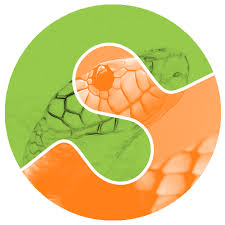
\includegraphics[height=0.075\textwidth]{fig/logos/python/scikit-image.jpeg}};
            \node[] at (.34,0.54) {
\includegraphics[height=0.075\textwidth]{fig/logos/python/scipy.png}};
            \node[] at (.2,0.565) {
\includegraphics[height=0.025\textwidth]{fig/logos/python/matplotlib.pdf}};
            \node[] at (.22,0.39) {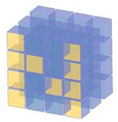
\includegraphics[height=0.075\textwidth]{fig/logos/python/numpy.png}};
        }
        \visible<1->{\node[] at (.28,0.48) {
\includegraphics[height=0.09\textwidth]{fig/logos/python/python.png}};}
        
        \visible<1->{
            \node[] at (.735,0.53) {
\includegraphics[height=0.075\textwidth]{fig/logos/imagej/trackmate.png}};
            \node[] at (.735,0.45) {
\includegraphics[height=0.075\textwidth]{fig/logos/imagej/fiji.png}};
            \node[] at (.658,0.375) {
\includegraphics[height=0.075\textwidth]{fig/logos/imagej/mammut.png}};
            \node[] at (.59,0.54) {
\includegraphics[height=0.075\textwidth]{fig/logos/imagej/imglib2.png}};
        }
        \visible<1->{\node[] at (.65,0.48) {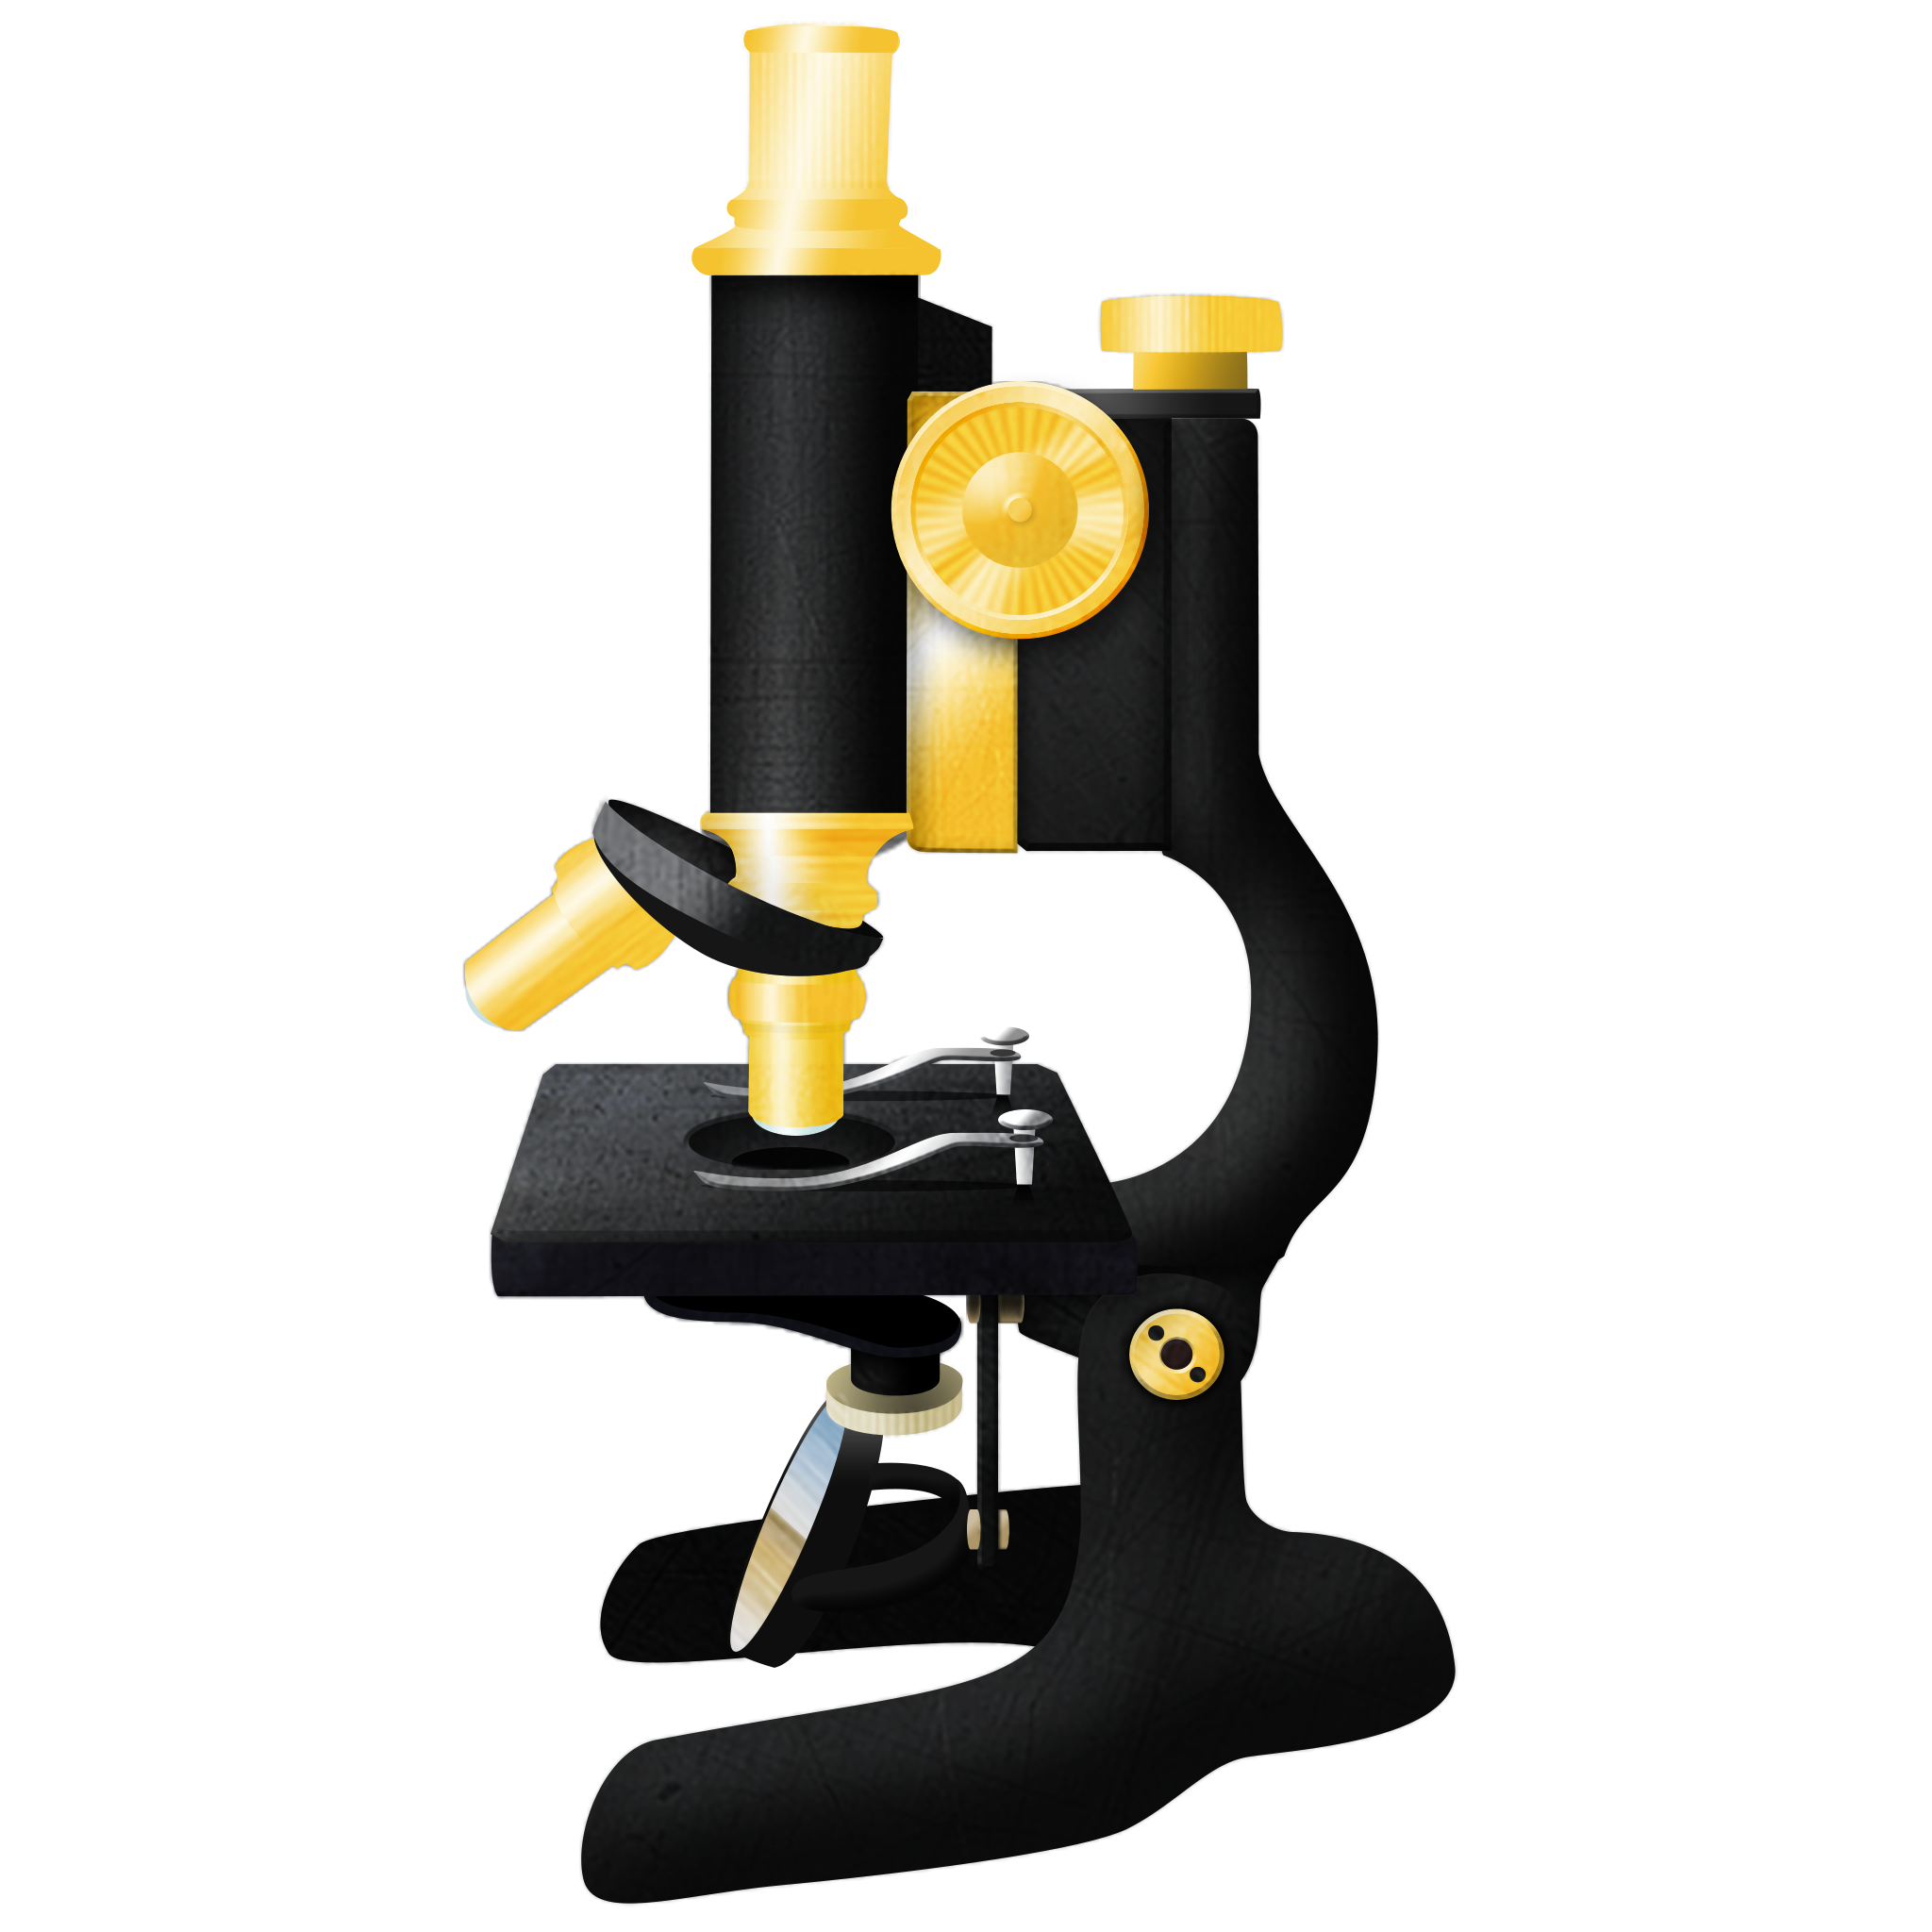
\includegraphics[height=0.13\textwidth]{fig/logos/imagej/imagej2.png}};}

        \visible<2->{
            % source https://openclipart.org/detail/209218/firebog-bridge
            \node[anchor=south west] at (0.38, 0.41) {
\includegraphics[width=0.19\linewidth]{fig/bridge.pdf}};
        }
        
    \end{tikzpicture}
\end{frame}

\begin{frame}[fragile]
    \frametitle{Installation \& Usage}
    \begin{itemize}
          \item<1-> Install imglyb from conda
        \begin{lstlisting}[language=bash]
conda install -c conda-forge imglyb
        \end{lstlisting}
          \item<2-> Install examples from PyPI
        \begin{lstlisting}[language=bash]
pip install imglyb-examples
        \end{lstlisting}
          \item<3-> Notebooks available on \mbox{\urlScrSz{https://github.com/hanslovsky/imglyb-learnathon}}
    \end{itemize}
\end{frame}

\begin{frame}[fragile]
    \frametitle{How to use?}
Import \lstinline[language=python,basicstyle=\ttfamily\normalsize]{imglyb}
    \begin{lstlisting}[language=python]
# import imglyb before jnius
import imglyb
from imglyb import util
# import from jnius what you need
from jnius import autoclass, cast, PythonJavaClass, java_method
    \end{lstlisting}
\end{frame}

\begin{frame}[fragile]
    \frametitle{Wrap NumPy arrays in ImgLib2}
    \begin{lstlisting}[language=python]
import imglyb
from imglyb import util

import numpy as np

img = np.random.rand( 300, 200, 100 ) * 2**16
wrapped = util.to_imglib( img )
util.BdvFunctions.show( wrapped, "wrapped image" )

rgba = np.random.randint( 
    2**32, size = ( 300, 200, 100 ), 
    dtype=np.uint32 )
wrapped_rgba = util.to_imglib_argb( rgba )
util.BdvFunctions.show( wrapped_rgba, "wrapped rgba image" )
    \end{lstlisting}

\end{frame}

\begin{frame}[fragile]
    \frametitle{Examples}
    Available in the imglyb-examples package:
    \begin{lstlisting}[language=bash]
imglyb-examples.bdv-hello-world
imglyb-examples.bdv-painter
imglyb-examples.butterfly
imglyb-examples.qt-awt
imglyb-examples.views-stack
    \end{lstlisting}
\end{frame}

\begin{frame}
    \frametitle{Example 1~--- BigDataViewer}
    BigDataViewer~(BDV) is a Java viewer for arbitrarily large multi-view 3D images and 3D image
    sequences developed by Tobias Pietzsch.
    
    \urlScrSz{https://imagej.net/BigDataViewer}
    
    \urlScrSz{https://github.com/hanslovsky/imglyb-learnathon/blob/master/notebooks/bdv/show-numpy-array-in-bdv.ipynb}
\end{frame}

\begin{frame}
    \frametitle{Example 2~--- BigDataViewer}
    BigDataViewer~(BDV) is a Java viewer for arbitrarily large multi-view 3D images and 3D image
    sequences developed by Tobias Pietzsch.
    
    \urlScrSz{https://imagej.net/BigDataViewer}
    
    \urlScrSz{https://github.com/hanslovsky/imglyb-learnathon/blob/master/notebooks/bdv/write-into-numpy-array-in-bdv.ipynb}
\end{frame}

\begin{frame}
    \frametitle{Example 3~--- BigWarp}
    BigWarp is a tool for interactive manual alignment of 2D or 3D images developed by John Bogovic.

    \urlScrSz{https://imagej.net/BigWarp}

    \urlScrSz{https://github.com/hanslovsky/imglyb-learnathon/blob/master/notebooks/bigwarp/bigwarp.ipynb}
\end{frame}

\begin{frame}
    \frametitle{Example 4~--- Paintera}
    Paintera is a tool for the fast generation of dense ground truth annotations and proof-reading
    3D EM connectomics with 3D visualization and mesh generation on the fly.

    \urlScrSz{https://github.com/saalfeldlab/paintera}

    \urlScrSz{https://github.com/hanslovsky/imglyb-learnathon/blob/master/notebooks/paintera/paintera-mesh-generation-on-the-fly.ipynb}
\end{frame}

\begin{frame}
    \frametitle{Known Issues}
    \begin{itemize}
          \item Java awt requires wrapper script on OSX
          \item Dask Arrays cannot be wrapped into ImgLib2 cell images
    \end{itemize}
\end{frame}

\begin{frame}
    \frametitle{Resources}
    \centering
    \vfill
    \begin{tabulary}{\linewidth}{lL}
        
\includegraphics[height=0.04\textwidth]{fig/logos/python/python.png} & \urlScrSz{https://www.python.org} \\
        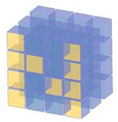
\includegraphics[height=0.04\textwidth]{fig/logos/python/numpy.png} & \urlScrSz{https://www.numpy.org} \\
        
\includegraphics[height=0.04\textwidth]{fig/logos/python/scipy.png} & \urlScrSz{https://scipy.org} \\
        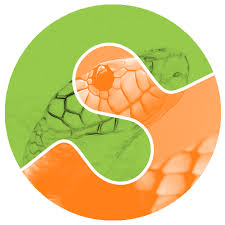
\includegraphics[height=0.04\textwidth]{fig/logos/python/scikit-image.jpeg} & \urlScrSz{https://scikit-image.org} \\
        
\includegraphics[height=0.04\textwidth]{fig/logos/python/matplotlib.pdf} & \urlScrSz{https://matplotlib.org} \\
        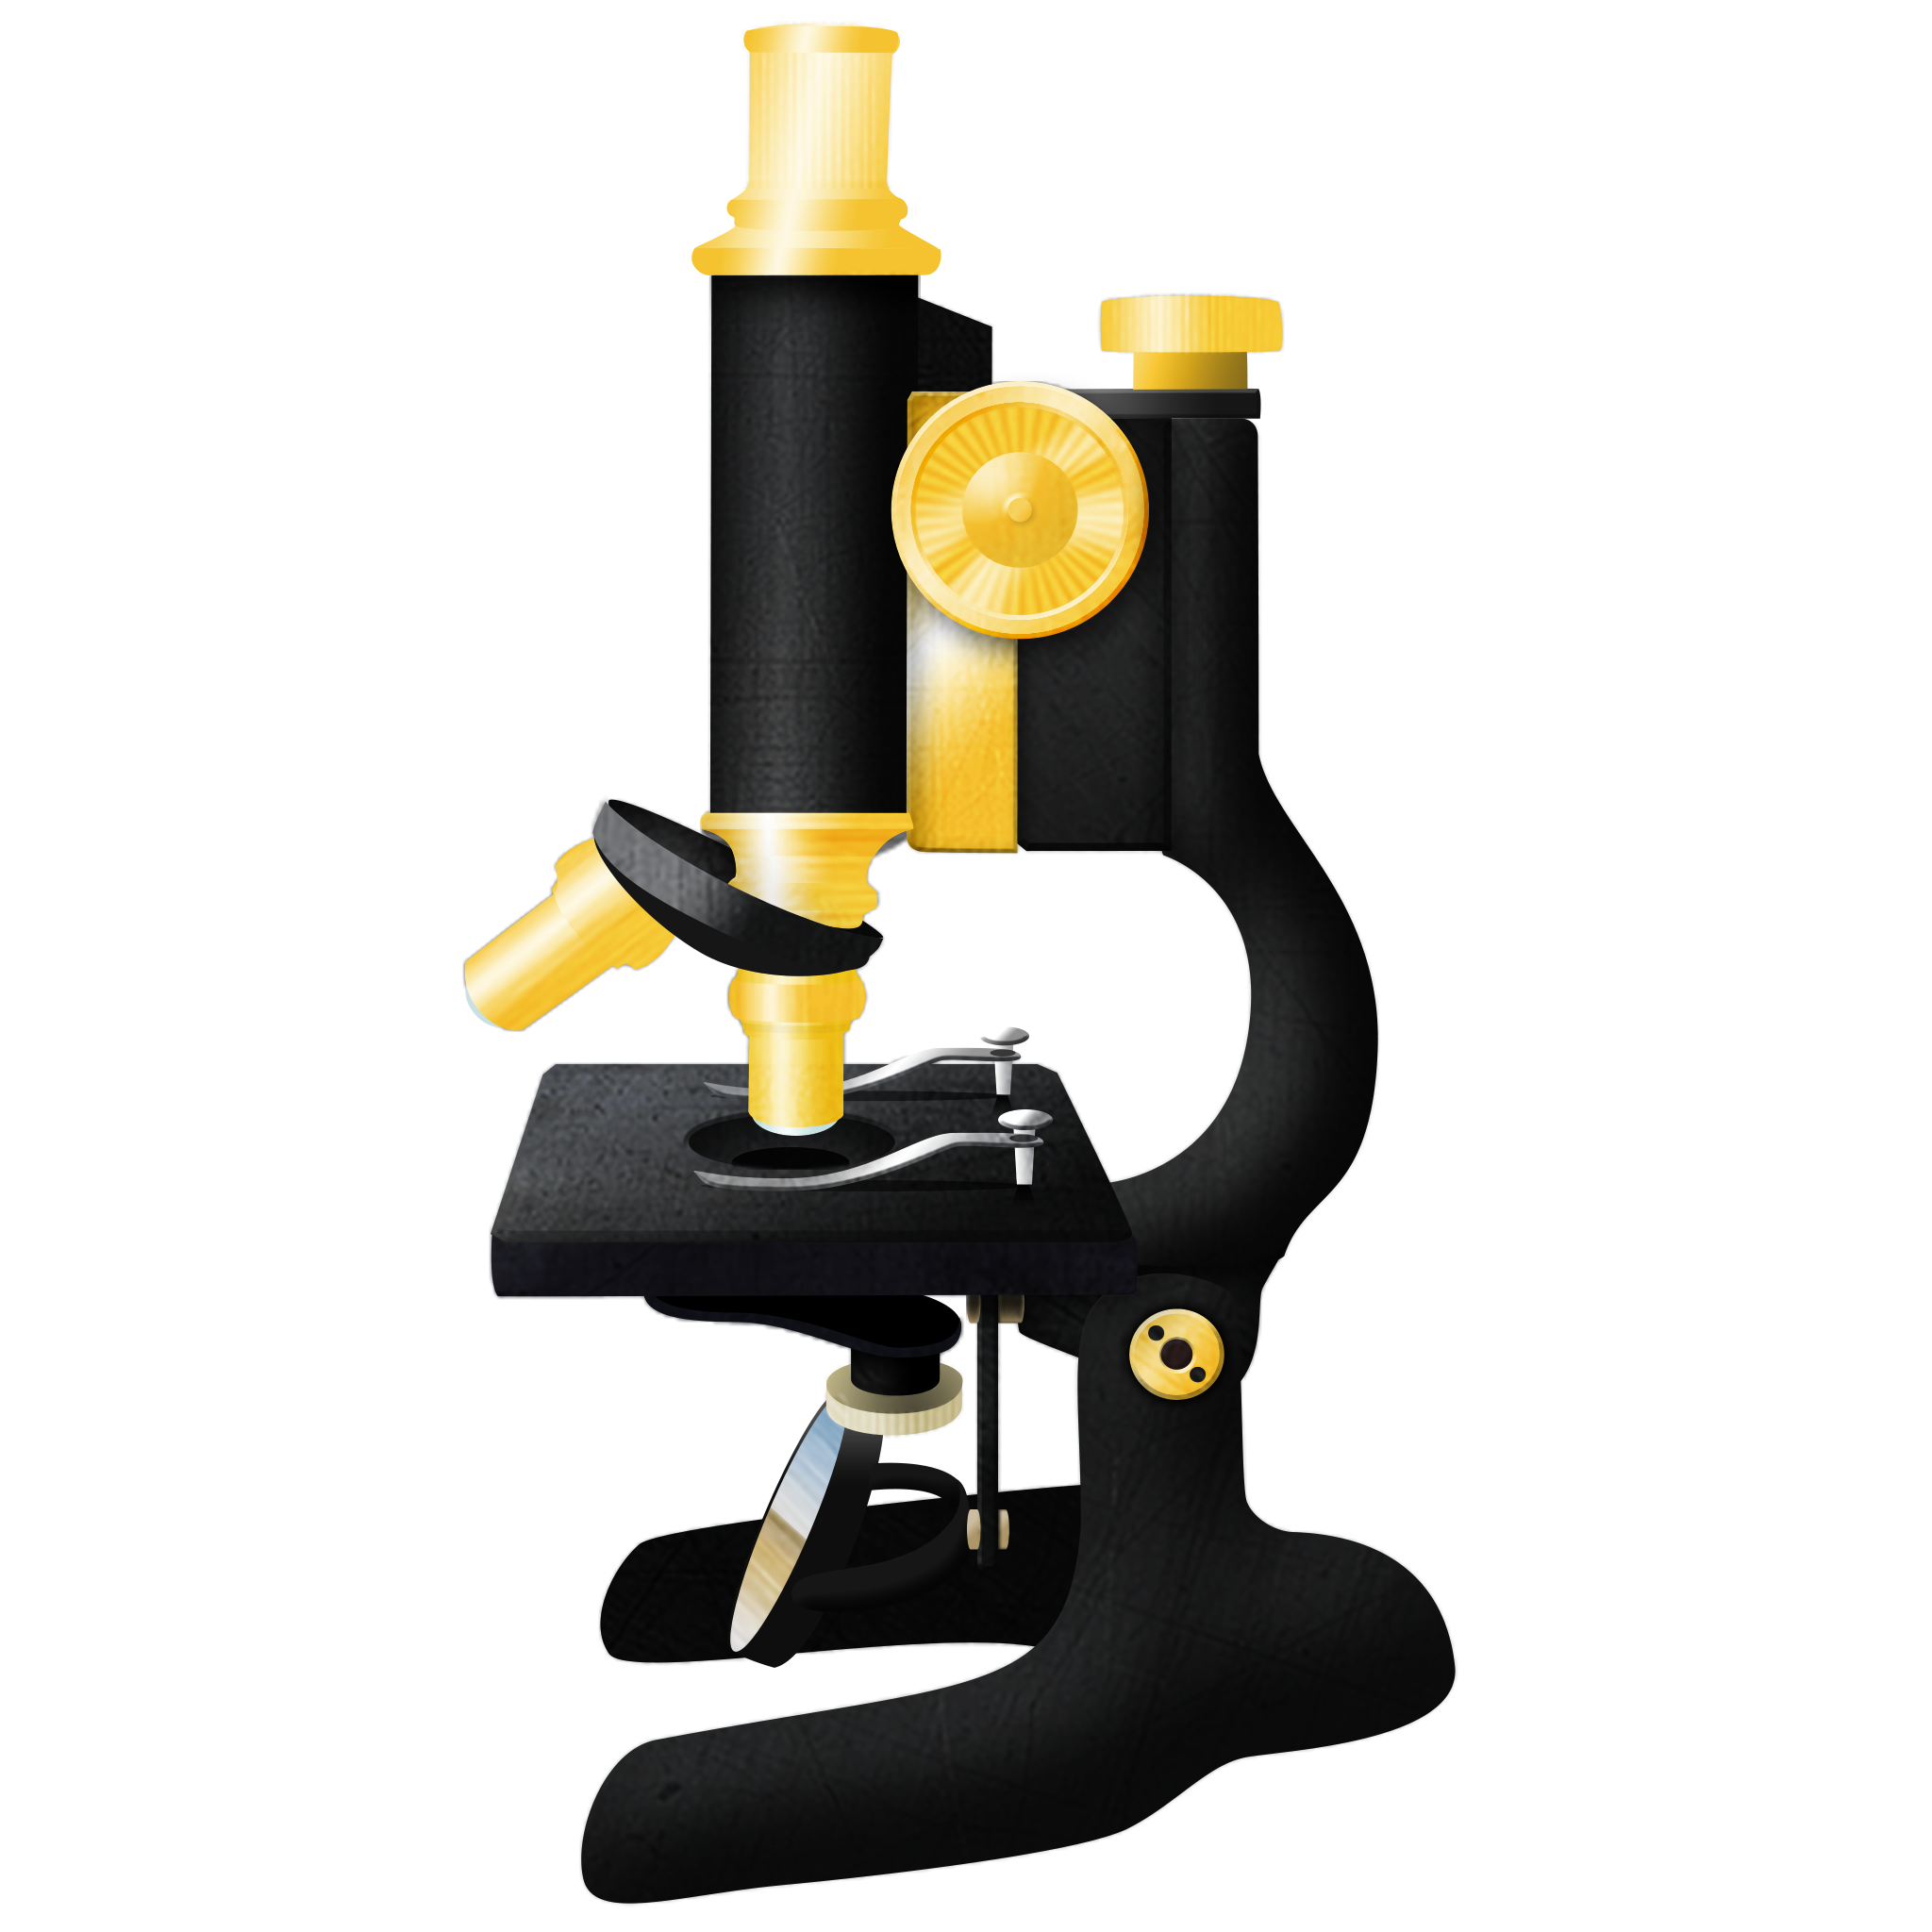
\includegraphics[height=0.04\textwidth]{fig/logos/imagej/imagej2.png} & \urlScrSz{https://imagej.net/ImageJ2} \\
        
\includegraphics[height=0.04\textwidth]{fig/logos/imagej/imglib2.png} & \urlScrSz{https://imagej.net/ImgLib2} \\
        
\includegraphics[height=0.04\textwidth]{fig/logos/imagej/trackmate.png} & \urlScrSz{https://imagej.net/TrackMate} \\
        
\includegraphics[height=0.04\textwidth]{fig/logos/imagej/fiji.png} & \urlScrSz{https://fiji.sc/} \\
        
\includegraphics[height=0.04\textwidth]{fig/logos/imagej/mammut.png} & \urlScrSz{https://imagej.net/MaMuT} \\
        
\includegraphics[height=0.04\textwidth]{fig/bridge.pdf} & \urlScrSz{https://openclipart.org/detail/209218/firebog-bridge}
    \end{tabulary}
\end{frame}

\begin{frame}[fragile]
    \frametitle{Thank You!}
\begin{lstlisting}[language=bash]
conda install -c conda-forge imglyb
pip install imglyb-examples
\end{lstlisting}
\urlScrSz{https://github.com/imglib/imglib2-unsafe}
\urlScrSz{https://github.com/imglib/imglib2-imglyb}
\urlScrSz{https://github.com/imglib/imglyb}
\urlScrSz{https://github.com/hanslovsky/imglyb-examples}
\urlScrSz{https://github.com/hanslovsky/imglyb-learnathon}
\urlScrSz{https://github.com/hanslovsky/scipy-2019}
\end{frame}

\end{document}

%%% Local Variables:
%%% mode: latex
%%% TeX-master: t
%%% End:
